\hypertarget{political-alignment-and-outlook}{%
\chapter{Political Alignment and
Outlook}\label{political-alignment-and-outlook}}

In the previous chapter, we used data from the General Social Survey
(GSS) to plot changes in political alignment over time. In this
notebook, we'll explore the relationship between political alignment and
respondents' beliefs about themselves and other people. We'll use the
following variables from the GSS dataset:

\begin{itemize}
\item
  \passthrough{\lstinline!happy!}: Taken all together, how would you say
  things are these days--would you say that you are very happy, pretty
  happy, or not too happy?
\item
  \passthrough{\lstinline!trust!}: Generally speaking, would you say
  that most people can be trusted or that you can't be too careful in
  dealing with people?
\item
  \passthrough{\lstinline!helpful!}: Would you say that most of the time
  people try to be helpful, or that they are mostly just looking out for
  themselves?
\item
  \passthrough{\lstinline!fair!}: Do you think most people would try to
  take advantage of you if they got a chance, or would they try to be
  fair?
\end{itemize}

We'll start with the last question; then as an exercise you can look at
one of the others. Here's the plan:

\begin{enumerate}
\def\labelenumi{\arabic{enumi}.}
\item
  First we'll use \passthrough{\lstinline!groupby!} to compare the
  average response between groups and plot the average as a function of
  time.
\item
  We'll use the Pandas function \passthrough{\lstinline!pivot table!} to
  compute the average response within each group as a function of time.
\item
  Finally, we'll use resampling to see whether the features we see in
  the results might be due to randomness, or whether they are likely to
  reflect actual changes in the works.
\end{enumerate}

I've created an HDF file that contains three
\passthrough{\lstinline!DataFrame!} objects with resampled GSS data.
We'll work with the first resampling, \passthrough{\lstinline!gss0!}, to
get started; at the end of this chapter, we'll see the other two as
well.

\begin{lstlisting}[]
datafile = "gss_pacs_resampled.hdf"
gss = pd.read_hdf(datafile, "gss0")
gss.shape
(@\dashfill@)
@@@(68846, 204)@@@
\end{lstlisting}

\hypertarget{are-people-fair}{%
\section{Are People Fair?}\label{are-people-fair}}

In the GSS data, the variable \passthrough{\lstinline!fair!} contains
responses to this question (see
\url{https://gssdataexplorer.norc.org/variables/440/vshow}):

\begin{quote}
Do you think most people would try to take advantage of you if they got
a chance, or would they try to be fair?
\end{quote}

The possible responses are:

\begin{lstlisting}
1   Take advantage
2   Fair
3   Depends
\end{lstlisting}

As always, we start by looking at the distribution of responses, that
is, how many people give each response:

\begin{lstlisting}[]
values(gss["fair"])
\end{lstlisting}

\begin{tabular}{lr}
\midrule
{} &   fair \\
\midrule
1.0 &  15435 \\
2.0 &  22806 \\
3.0 &   2755 \\
\midrule
\end{tabular}

The plurality think people try to be fair (2), but a substantial
minority think people would take advantage (1). There are also a number
of NaNs, mostly respondents who were not asked this question.

\begin{lstlisting}[]
gss["fair"].isna().sum()
(@\dashfill@)
@@@27850@@@
\end{lstlisting}

To count the number of people who chose option 2, ``people try to be
fair'', we'll use a dictionary to recode option 2 as
\passthrough{\lstinline!1!} and the other options as
\passthrough{\lstinline!0!}.

\begin{lstlisting}[]
recode_fair = {1: 0, 2: 1, 3: 0}
\end{lstlisting}

As an alternative, we could include option 3, ``depends'', by mapping it
to 1, or give it less weight by mapping it to an intermediate value like
0.5.

We can use \passthrough{\lstinline!replace!} to recode the values and
store the result as a new column in the DataFrame.

\begin{lstlisting}[]
gss["fair2"] = gss["fair"].replace(recode_fair)
\end{lstlisting}

And we'll use \passthrough{\lstinline!values!} to check whether it
worked.

\begin{lstlisting}[]
values(gss["fair2"])
\end{lstlisting}

\begin{tabular}{lr}
\midrule
{} &  fair2 \\
\midrule
0.0 &  18190 \\
1.0 &  22806 \\
\midrule
\end{tabular}

\hypertarget{fairness-over-time}{%
\section{Fairness Over Time}\label{fairness-over-time}}

As we saw in the previous notebook, we can use
\passthrough{\lstinline!groupby!} to group responses by year.

\begin{lstlisting}[]
gss_by_year = gss.groupby("year")
\end{lstlisting}

From the result we can select \passthrough{\lstinline!fair2!} and
compute the mean.

\begin{lstlisting}[]
fair_by_year = gss_by_year["fair2"].mean()
\end{lstlisting}

Here's the result, which shows the fraction of people who say people try
to be fair, plotted over time. As in the previous notebook, we plot the
data points themselves with circles and a local regression model as a
line.

\begin{lstlisting}[]
plot_series_lowess(fair_by_year, "C1")

decorate(
    xlabel="Year",
    ylabel="Fraction saying yes",
    title="Would most people try to be fair?",
)
\end{lstlisting}

\begin{center}
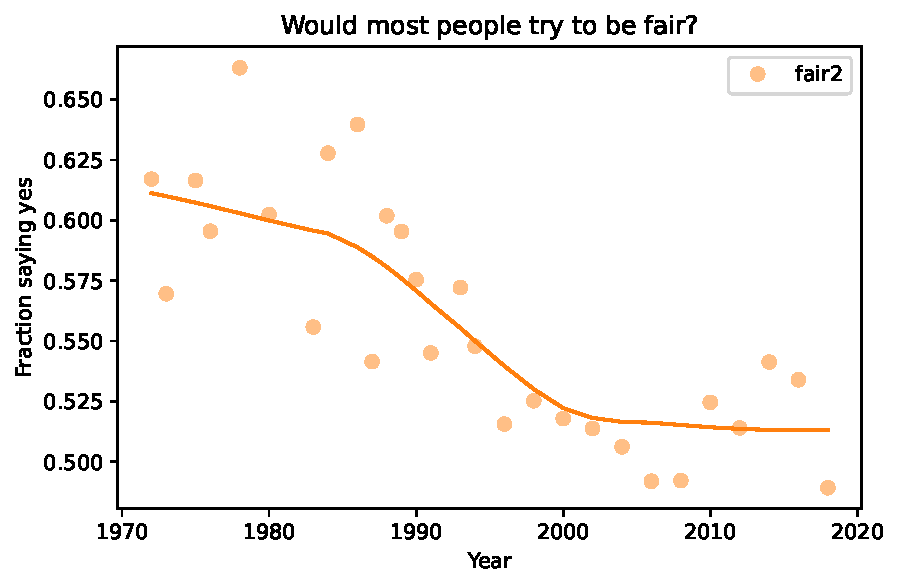
\includegraphics[width=4in]{chapters/03_outlook_files/03_outlook_31_0.pdf}
\end{center}

Sadly, it looks like faith in humanity has declined, at least by this
measure.

Let's see what this trend looks like if we group the respondents by
political alignment.

\hypertarget{political-views-on-a-3-point-scale}{%
\section{Political Views on a 3-point
Scale}\label{political-views-on-a-3-point-scale}}

In the previous notebook, we looked at responses to
\passthrough{\lstinline!polviews!}, which asks about political
alignment. The valid responses are:

\begin{lstlisting}
1   Extremely liberal
2   Liberal
3   Slightly liberal
4   Moderate
5   Slightly conservative
6   Conservative
7   Extremely conservative
\end{lstlisting}

To make it easier to visualize groups, we'll lump the 7-point scale into
a 3-point scale.

\begin{lstlisting}[]
recode_polviews = {
    1: "Liberal",
    2: "Liberal",
    3: "Liberal",
    4: "Moderate",
    5: "Conservative",
    6: "Conservative",
    7: "Conservative",
}
\end{lstlisting}

We'll use \passthrough{\lstinline!replace!}, as we've seen before, and
store the result as a new column in the DataFrame.

\begin{lstlisting}[]
gss["polviews3"] = gss["polviews"].replace(recode_polviews)
\end{lstlisting}

With this scale, there are roughly the same number of people in each
group.

\begin{lstlisting}[]
values(gss["polviews3"])
\end{lstlisting}

\begin{tabular}{lr}
\midrule
{} &  polviews3 \\
\midrule
Conservative &      20359 \\
Liberal      &      16195 \\
Moderate     &      22950 \\
\midrule
\end{tabular}

\hypertarget{fairness-by-group}{%
\section{Fairness by Group}\label{fairness-by-group}}

Now let's see who thinks people are more fair, conservatives or
liberals. We'll group the respondents by
\passthrough{\lstinline!polviews3!}.

\begin{lstlisting}[]
by_polviews = gss.groupby("polviews3")
\end{lstlisting}

And compute the mean of \passthrough{\lstinline!fair2!} in each group.

\begin{lstlisting}[]
by_polviews["fair2"].mean()
\end{lstlisting}

\begin{tabular}{lr}
\midrule
{} &     fair2 \\
polviews3    &           \\
\midrule
Conservative &  0.582789 \\
Liberal      &  0.553916 \\
Moderate     &  0.542407 \\
\midrule
\end{tabular}

It looks like conservatives are a little more optimistic, in this sense,
than liberals and moderates. But this result is averaged over the last
50 years. Let's see how things have changed over time.

\hypertarget{fairness-over-time-by-group}{%
\section{Fairness over Time by
Group}\label{fairness-over-time-by-group}}

So far, we have grouped by \passthrough{\lstinline!polviews3!} and
computed the mean of \passthrough{\lstinline!fair2!} in each group. Then
we grouped by \passthrough{\lstinline!year!} and computed the mean of
\passthrough{\lstinline!fair2!} for each year. Now I want to group by
\passthrough{\lstinline!polviews3!} and \passthrough{\lstinline!year!},
and compute the mean of \passthrough{\lstinline!fair2!} in each group
over time.

We could do that computation ``by hand'' using the tools we already
have, but it is so common and useful that it has a name: it is called a
\textbf{pivot table}, and Pandas provides a function that computes it
(see
\url{https://pandas.pydata.org/pandas-docs/stable/reference/api/pandas.pivot_table.html}).

The function is called \passthrough{\lstinline!pivot\_table!}, and it
takes the following arguments:

\begin{itemize}
\item
  \passthrough{\lstinline!values!}, which is the name of the variable we
  want to summarize: \passthrough{\lstinline!fair2!} in this example.
\item
  \passthrough{\lstinline!index!}, which is the name of the variable
  that will provide the row labels: \passthrough{\lstinline!year!} in
  this example.
\item
  \passthrough{\lstinline!columns!}, which is the name of the variable
  that will provide the column labels:
  \passthrough{\lstinline!polview3!} in this example.
\item
  \passthrough{\lstinline!aggfunc!}, which is the function used to
  ``aggregate'', or summarize, the values:
  \passthrough{\lstinline!mean!} in this example.
\end{itemize}

\begin{lstlisting}[]
table = gss.pivot_table(
    values="fair2", index="year", columns="polviews3", aggfunc="mean"
)
\end{lstlisting}

The result is a table that has years running down the rows and political
alignment running across the columns. Each entry in the table is the
mean of \passthrough{\lstinline!fair2!} for a given group in a given
year.

\begin{lstlisting}[]
table.head()
\end{lstlisting}

\begin{tabular}{lrrr}
\midrule
polviews3 &  Conservative &   Liberal &  Moderate \\
year &               &           &           \\
\midrule
1975 &      0.625616 &  0.617117 &  0.647280 \\
1976 &      0.631696 &  0.571782 &  0.612100 \\
1978 &      0.694915 &  0.659420 &  0.665455 \\
1980 &      0.600000 &  0.554945 &  0.640264 \\
1983 &      0.572438 &  0.585366 &  0.463492 \\
\midrule
\end{tabular}

Reading across the first row, we can see that in 1975, moderates were
slightly more optimistic than the other groups.

Reading down the first column, we can see that the estimated mean of
\passthrough{\lstinline!fair2!} among conservatives varies from year to
year. It is hard to tell looking at these numbers whether it is trending
up or down; we can get a better view by plotting the results.

\hypertarget{plotting-the-results}{%
\section{Plotting the Results}\label{plotting-the-results}}

We can use \passthrough{\lstinline!plot\_columns\_lowess!} to see the
results.

\begin{lstlisting}[]
columns = ["Conservative", "Liberal", "Moderate"]
plot_columns_lowess(table, columns, colors)

decorate(
    xlabel="Year",
    ylabel="Fraction saying yes",
    title="Would most people try to be fair?",
)
\end{lstlisting}

\begin{center}
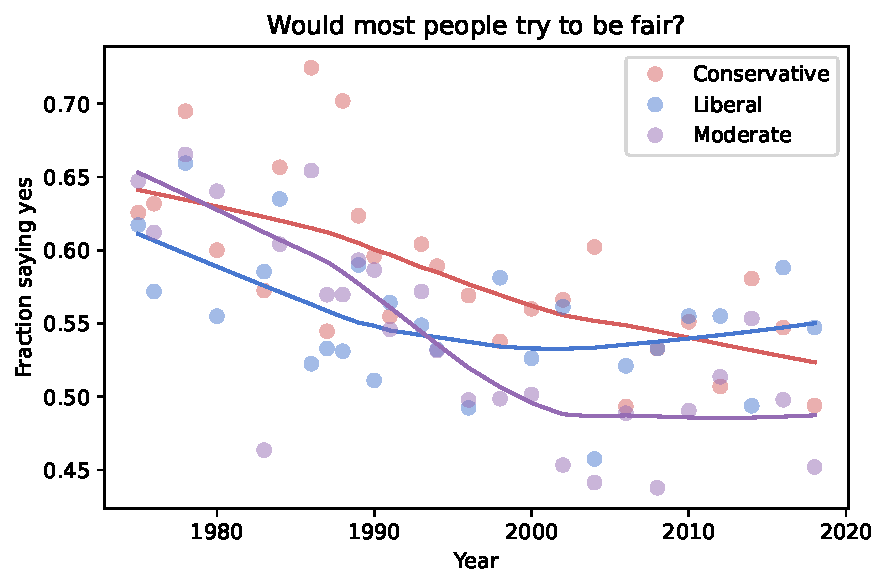
\includegraphics[width=4in]{chapters/03_outlook_files/03_outlook_54_0.pdf}
\end{center}

The fraction of respondents who think people try to be fair has dropped
in all three groups, although liberals and moderates might have leveled
off. In 1975, liberals were the least optimistic group. In 2018, they
might be the most optimistic. But the responses are quite noisy, so we
should not be too confident about these conclusions.

We can get a sense of how reliable they are by running the resampling
process a few times and checking how much the results vary.

\hypertarget{simulating-possible-datasets}{%
\section{Simulating Possible
Datasets}\label{simulating-possible-datasets}}

The figures we have generated so far in this notebook are based on a
single resampling of the GSS data. Some of the features we see in these
figures might be due to random sampling rather than actual changes in
the world.

By generating the same figures with different resampled datasets, we can
get a sense of how much variation there is due to random sampling.

To make that easier, the following function contains the code from the
previous analysis all in one place.

\begin{lstlisting}[]
def plot_by_polviews(gss):
    """Plot mean response by polviews and year.

    gss: DataFrame
    """
    gss["polviews3"] = gss["polviews"].replace(recode_polviews)
    gss["fair2"] = gss["fair"].replace(recode_fair)

    table = gss.pivot_table(
        values="fair2", index="year", columns="polviews3", aggfunc="mean"
    )

    plot_columns_lowess(table, columns, colors)

    decorate(
        xlabel="Year",
        ylabel="Fraction saying yes",
        title="Would most people try to be fair?",
    )
\end{lstlisting}

Now we can loop through the three resampled datasets in the HDF5 file
and generate a figure for each one.

\begin{lstlisting}[]
datafile = "gss_pacs_resampled.hdf"

for key in ["gss0", "gss1", "gss2"]:
    df = pd.read_hdf(datafile, key)

    plt.figure()
    plot_by_polviews(df)
\end{lstlisting}

\begin{center}
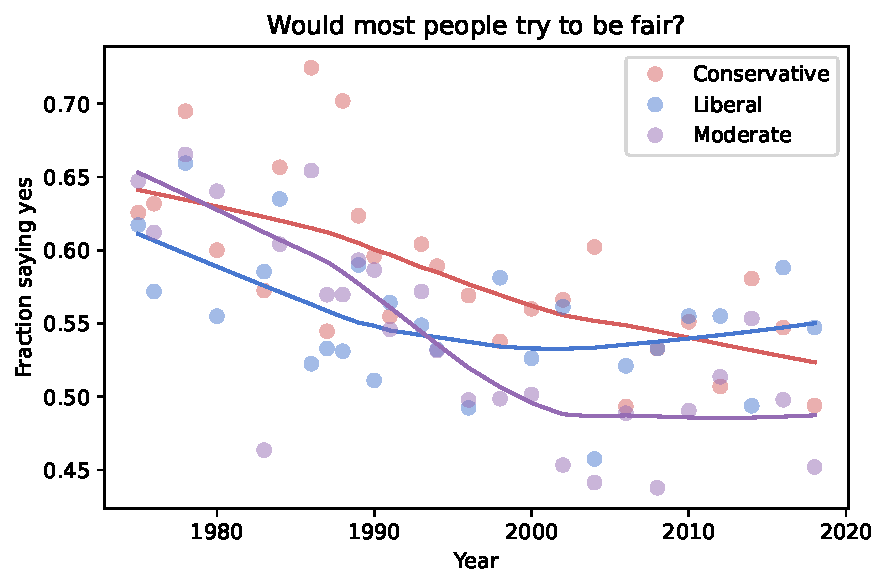
\includegraphics[width=3in]{chapters/03_outlook_files/03_outlook_59_0.pdf}
\end{center}

\begin{center}
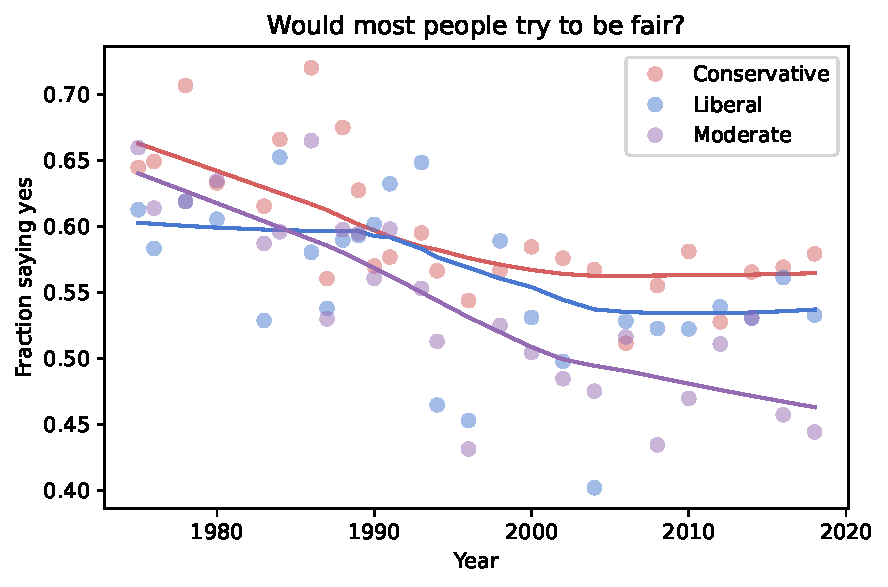
\includegraphics[width=3in]{chapters/03_outlook_files/03_outlook_59_1.pdf}
\end{center}

\begin{center}
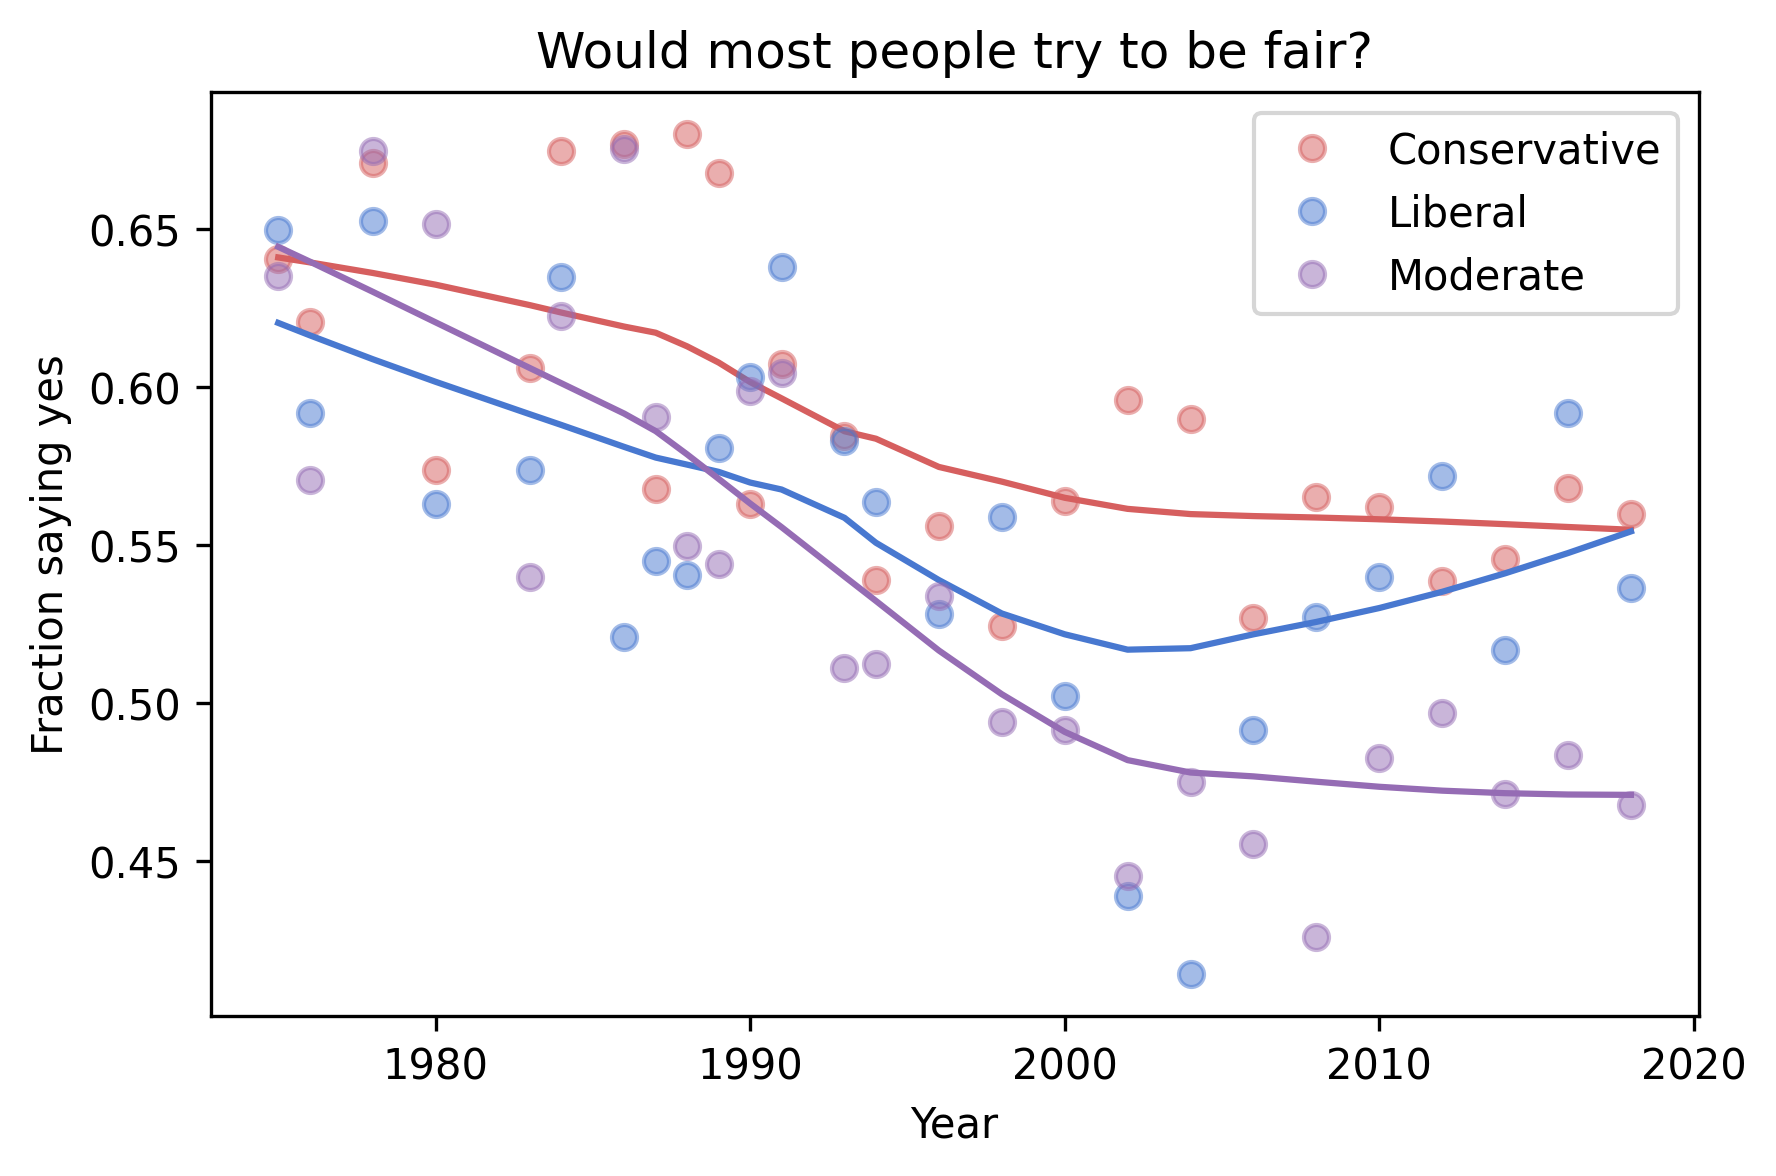
\includegraphics[width=3in]{chapters/03_outlook_files/03_outlook_59_2.png}
\end{center}

Features that are the same in all three figures are more likely to
reflect things actually happening in the world. Features that differ
substantially between the figures are more likely to be artifacts of
random sampling. In this context, ``artifact'' has the sense of
``something observed in a scientific investigation or experiment that is
not naturally present but occurs as a result of the preparative or
investigative procedure'' (from
\url{https://www.lexico.com/en/definition/artifact}).

\textbf{Exercise:} As an exercise, you can run the same analysis with
one of the other variables related to outlook including
\passthrough{\lstinline!happy!}, \passthrough{\lstinline!trust!},
\passthrough{\lstinline!helpful!}, and maybe
\passthrough{\lstinline!fear!} and \passthrough{\lstinline!hapmar!}.

For these variables, you will have to read the codebook to see the
responses and how they are encoded, then think about which responses to
report. In the notebook for this chapter, there are some suggestions to
get you started.

\hypertarget{summary}{%
\section{Summary}\label{summary}}

The case study in this chapter and the previous one demonstrates a
process for exploring a dataset and finding relationships among the
variables.

In the previous chapter, we started with a single variable,
\passthrough{\lstinline!polviews!}, and visualized its distribution at
the beginning and end of the observation interval. Then we used
\passthrough{\lstinline!groupby!} to see how the mean and standard
deviation changed over time. Looking more closely, we used cross
tabulation to see how the fraction of people in each group changed over
time.

In this chapter, we added a second variable,
\passthrough{\lstinline!fair!}, which is one of several questions in the
GSS related to respondents' beliefs about other people. We used
\passthrough{\lstinline!groupby!} again to see how the responses have
changed over time. Then we used a pivot table to show how the responses
within each political group have changed over time. Finally, we used
multiple resamplings of the original dataset to check whether the
patterns we identified might be due to random sampling rather than real
changes in the world.

The tools we used in this case study are versatile; they are useful for
exploring other variables in the GSS dataset, and other datasets as
well. And the process we followed is one I recommend whenever you are
exploring a new dataset.

